\documentclass[a4paper,10pt]{article}
\usepackage{fontspec}
\defaultfontfeatures{Mapping=tex-text,Ligatures=TeX}
\usepackage[inner=3cm,top=3cm,outer=3cm,bottom=3cm]{geometry}
\usepackage[parfill]{parskip}
\usepackage{csquotes}
\usepackage{amsmath}
\usepackage{amssymb}
\usepackage{mathtools}
\usepackage{verbatim}
\usepackage{algpseudocode}
\usepackage{float}
\usepackage{tikz}
\usepackage{mathtools}
\usepackage[backend=biber,style=numeric]{biblatex}
\usepackage{pgfgantt}
\addbibresource{references/bibliography.bib}
\DeclarePairedDelimiter\ceil{\lceil}{\rceil}
\DeclarePairedDelimiter\floor{\lfloor}{\rfloor}

\newcommand{\cauthor}{André Nyström \& Axel Riese}
\newcommand{\ctitle}{Algorithms and Complexity for Video and Computer Games}
\newcommand{\csubtitle}{A Lumines survey}
\newcommand{\cdate}{\today}
\newcommand{\caddress}
{
    Degree Project in Computer Science, DD143X \\
    Examinator: Örjan Ekeberg
}


\title{Algorithms and Complexity for Video and Computer Games \\
    \textit{Project Specification}} % Title
\author{\cauthor} % Author name
\date{\today} % Date for the report

\begin{document}
\maketitle % Insert the title, author and date

\section{Introduction}
Our chosen general subject is algorithms and complexity in computer games, specifically the 2004 puzzle game ``Lumines''. Our project will concern the computational complexity of one or several goals related to playing the game.

The subject is of interest because Lumines is to our knowledge not very well researched when it comes to computational complexity. Similar puzzle games, such as Tetris, Bejeweled and Puyo puyo has been more thoroughly examined in recent years, and it seems interesting to us how Lumines will compare. While these findings may seem to be of lesser importance, they may teach us more about the nature of computational complexity, or aid in reductions to other problem instances.

\section{Problem statement}
The essence of Lumines is to create as many $2 \times 2$ monochromatic squares (blocks) as possible, using a particular sequence of $2 \times 2$ dichromatic squares (pieces).

The problem we want to answer is ``Is Lumines NP-complete?''. More specifically, we want to focus our attention on the problem of maximizing the number of blocks one can create using a priorly known sequence of pieces and an initial gameboard. 

\section{Approach}
Our approach to the problem is at first to simplify the game mechanics, for example we will probably consider the ``sweep mechanic'' of the game to be instantaneous instead of moving. We will also consider the offline version of the game, where every piece involved in a game sessions is known beforehand, rather than the actual online version, where the game pieces are generated probabilistically.

We will then start to define the rules of the game in a rigorous manner. Once we have a mathematical system, we can proceed to formulate a decision problem of interest in that system. After this is done, we can try to prove that the problem is in fact NP-complete. This is done in the standard way; we will first try show that the problem is in NP, by proving that an answer is verifiable in polynomial time, and then try find a suitably reduction from a known NP-complete problem to our problem at hand.

Lastly, if time permits, we can change the rules of our system to be more true to the actual game. For example we could consider continuous sweeps, piece drop speed simulation and online versions of the game. We will then try to prove our previous findings in this new system, which will hopefully tell us more about the original game.

\section{References}
So far we have identified three papers which we consider relevant for our project. One these is a description of Lumines strategies \cite{lumines}, the remaining two regards computational complexity in Tetris \cite{tetris} and Match-three puzzle games \cite{candy}. The Tetris paper is especially of interest. The paper describes a good method for how to approach reasoning about computational complexity in a video game context, such as formalizing the rules of the game in a mathematical system. The fact that Tetris and Lumines share some characteristics, but are not fully alike, makes it possible for us to be inspired by the paper, but not to the point of plagiarism.

\newcommand\Dganttbar[4]{%
  \ganttbar{#1}{#3}{#4}\ganttbar[inline,bar label font=\footnotesize]{#2}{#3}{#4}
}

\section{Time plan}
 \begin{figure}[H]
    \centering
    \resizebox{\textwidth}{!} {
    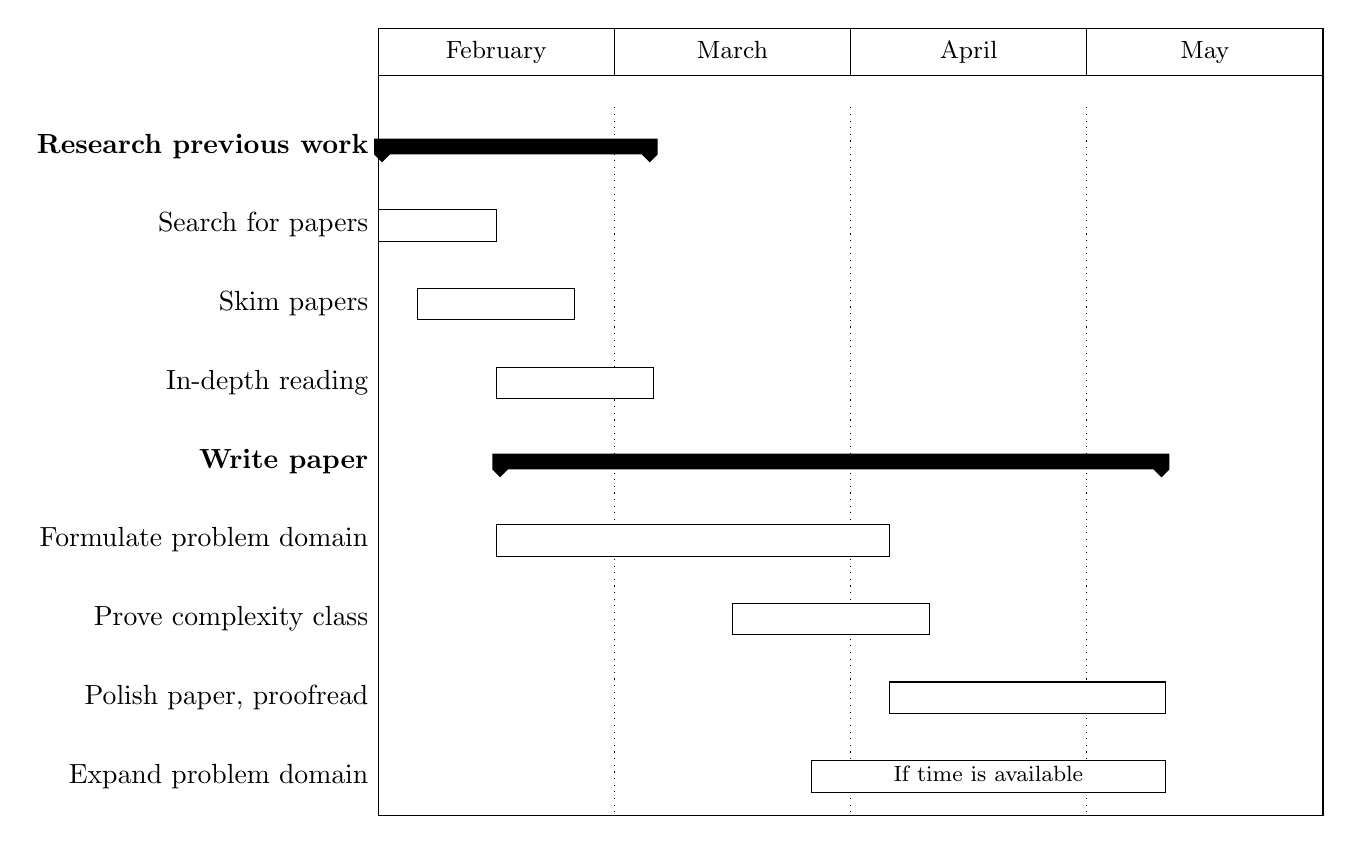
\begin{tikzpicture}[transform shape]
    \begin{ganttchart}[
        vgrid={draw=none, draw=none, draw=none, draw=none, draw=none, dotted}
    ]{1}{24}
      \gantttitle{February}{6} 
      \gantttitle{March}{6} 
      \gantttitle{April}{6} 
      \gantttitle{May}{6} \\
    \ganttgroup{Research previous work}{1}{7} \\
    \ganttbar{Search for papers}{1}{3} \\
    \ganttbar{Skim papers}{2}{5} \\
    \ganttbar{In-depth reading}{4}{7} \\
    \ganttgroup{Write paper}{4}{20} \\
    \ganttbar{Formulate problem domain}{4}{13} \\
    \ganttbar{Prove complexity class}{10}{14} \\
    \ganttbar{Polish paper, proofread}{14}{20} \\
    \ganttbar{Expand problem domain}{12}{20}
    \ganttbar[inline, bar label font=\footnotesize]{If time is available}{12}{20}
    \end{ganttchart}
    \end{tikzpicture}
    }
    \textit{Time plan as a Gantt chart}
\end{figure}
\printbibliography
\end{document}
